\begin{figure*}

\begin{minipage}{0.65\textwidth}
  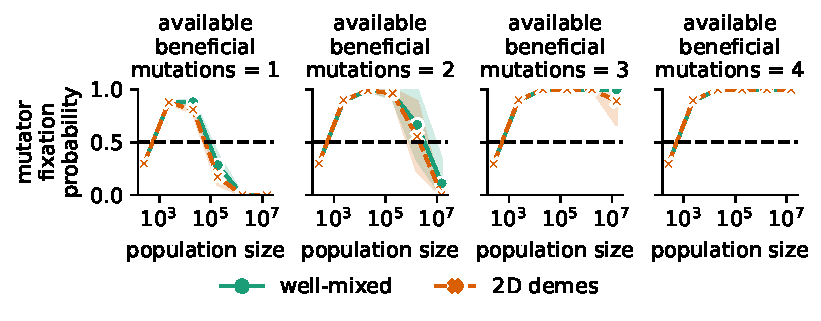
\includegraphics[width=\textwidth]{binder/binder-cupy-5050-traits.ipynb/binder/teeplots/cupy-5050-traits/col=available-beneficial-mutations+errorbar=ci+hue=population-structure+kind=line+palette=dark2+style=population-structure+viz=relplot+x=population-size+y=fixation-probability+ext=.pdf}%
\end{minipage}
\begin{minipage}{0.3\textwidth}
\caption{
\textbf{Well-mixed and spatially-structured populations exhibit similar relationship between population size and mutator fixation probability in 50/50 competition experiments.}
\footnotesize
In both scenarios, as available beneficial mutations are increased, mutators gain favor in progressively larger population sizes.
Simulations were conducted on GPU using the counter-based genome model, with populations initialized to a 50/50 mix of non- and mutators.
Subpopulations comprised 256 agents per PE.
Shaded bands show bootstrapped 95\% confidence intervals.
}
\label{fig:avail-ben-muts-gen}
\end{minipage}

\end{figure*}
